\section{Evaluation}
To evaluate the impact flat combining has on the global data structures, we ran a series of experiments to test the raw performance of the data structures themselves under different workloads, and further measured their impact on performance of two simple graph benchmarks.

Experiments were run on a cluster of AMD Interlagos processors. Nodes have 32 2.1-GHz cores in two sockets, 64GB of memory, and 40Gb Mellanox ConnectX-2 InfiniBand network cards, connected via a QLogic InfiniBand switch.

\subsection{Data Structure Throughput}
First we measured the raw performance of the global data structures on extremely simple throughput workloads.

% \begin{figure*}[t]
%   \centering
\begin{figure}[t] %{0.5\textwidth}
  \centering
  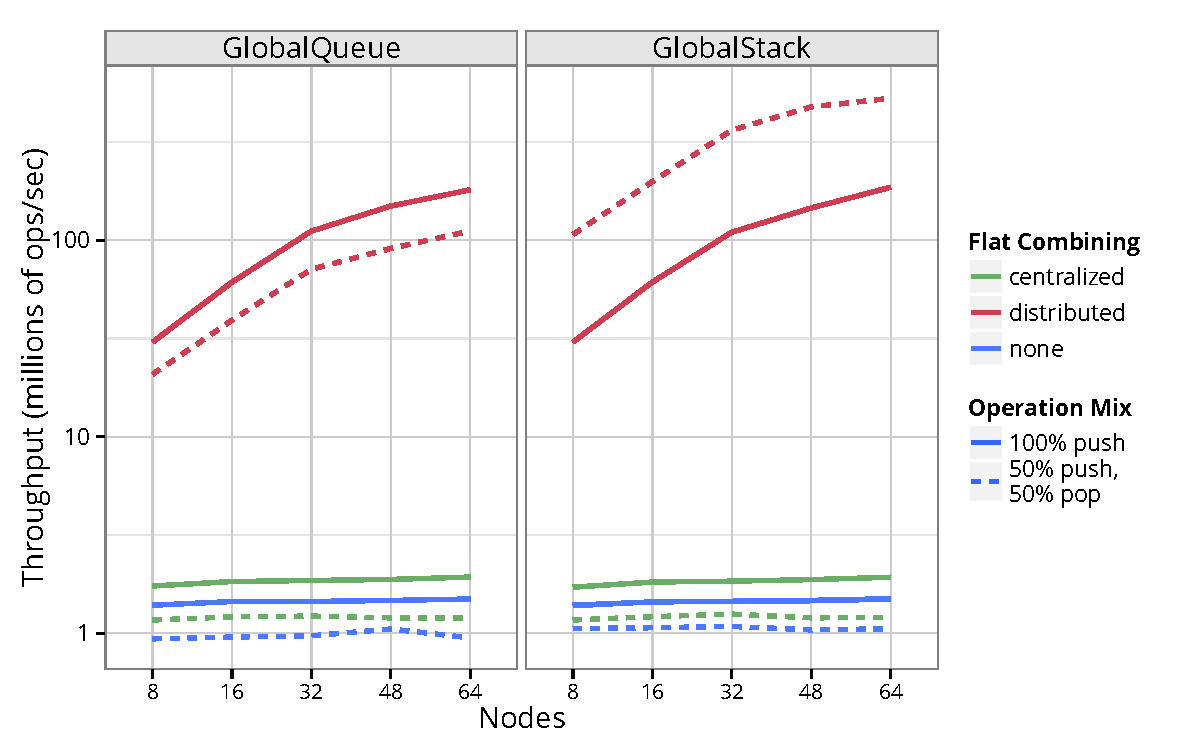
\includegraphics[width=0.5\textwidth]{data/plots/vector_perf.pdf}
  \caption{\emph{GlobalStack and GlobalQueue.}
    Results are shown on a log scale for a throughput workload performing 256 million operations with 2048 workers per core and 16 cores per node. Flat combining improves throughput by at least an order of magnitude and allows performance to scale. Matching pushes and pops enables the stack to perform even better on a mixed workload.
  }
  \label{fig:vector}
\end{figure}
  % \hspace{0.05\textwidth}
  % % ~ %add desired spacing between images, e. g. ~, \quad, \qquad etc.
  % %(or a blank line to force the subfigure onto a new line)
  % \begin{subfigure}[b]{0.45\textwidth}
  % \centering
  % 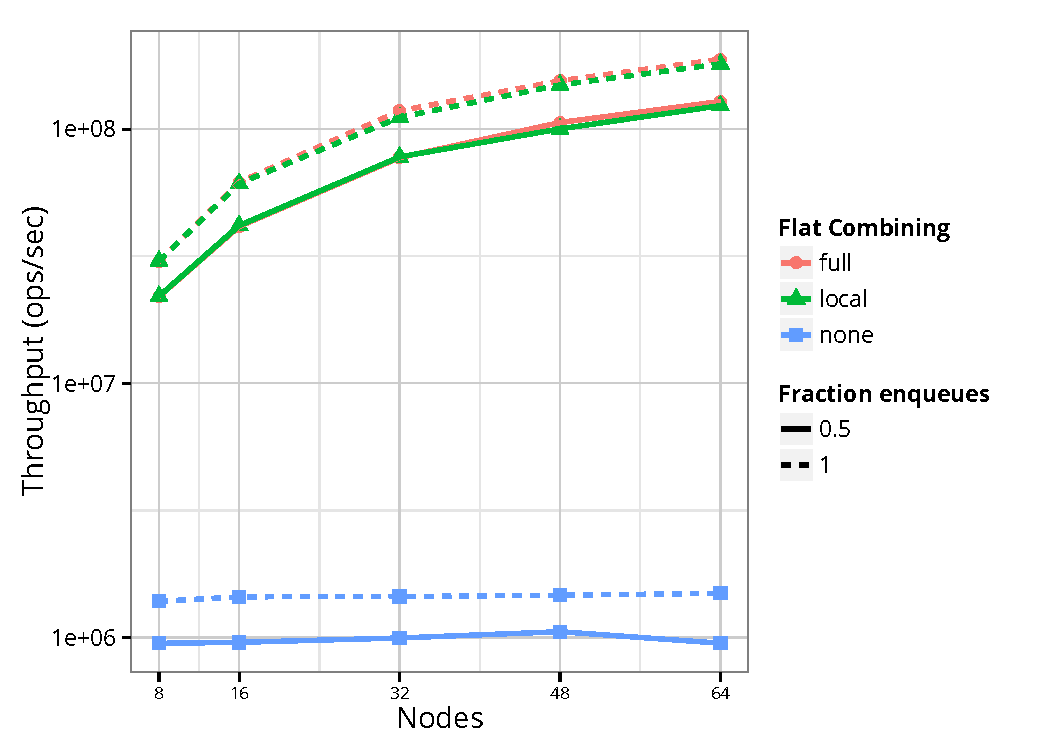
\includegraphics[width=\textwidth]{data/plots/queue_perf.pdf}
  % \caption{\emph{GlobalQueue.} Same parameters as stack performance results. The queue is unable to do matching locally, but benefits from reducing the amount of synchronization that must globally serialize. The mixed workload performs worse because the current implementation serializes combined enqueue and dequeue operations.}
  % \label{fig:queue}
  % \end{subfigure}
  % \hspace{0.05\textwidth}
  
  %  
\begin{figure}[t]
  \centering
  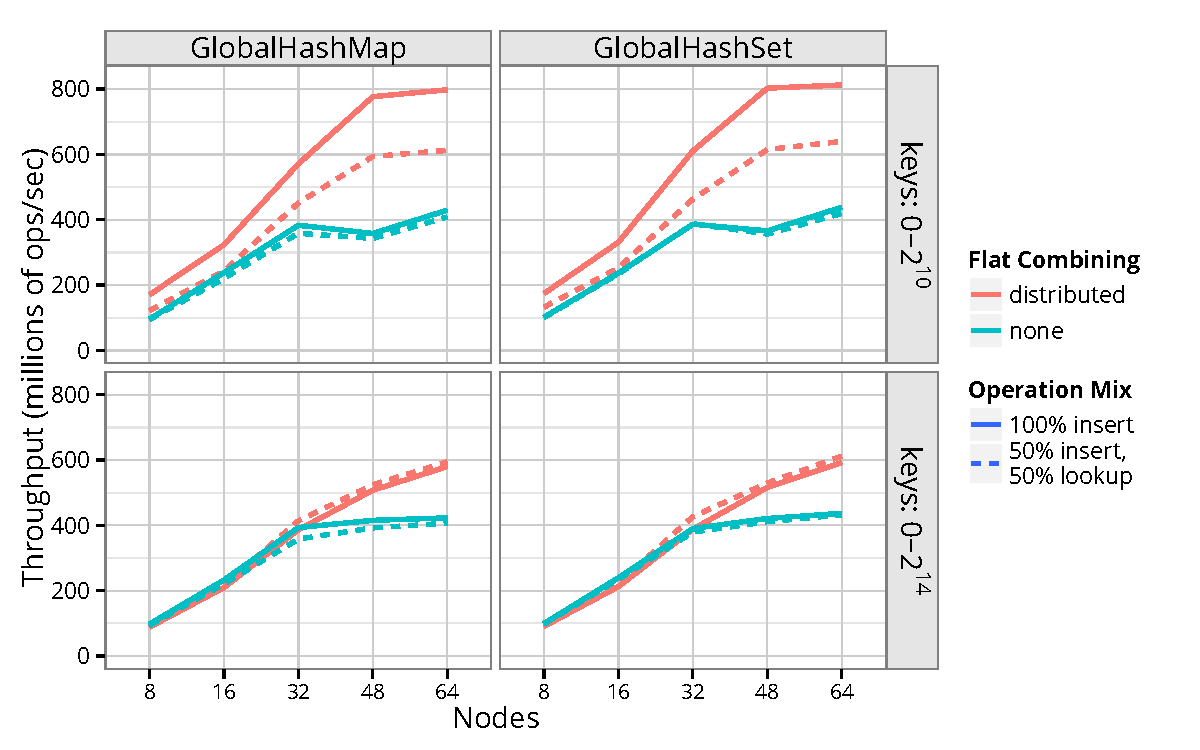
\includegraphics[width=0.5\textwidth]{data/plots/hash_perf.pdf}
  \caption{\emph{GlobalHashSet and GlobalHashMap.}
    Results are shown for a throughput workload inserting and looking up 256 million random keys in the range 0-1024 into a global hash with 1024 cells, with 2048 workers per core and 16 cores per node.
    Performance without combining scales out to 32 nodes because synchronization happens at each hash cell, but drops off as the number of destinations increases. Due to eliminating duplicate inserts and lookups, the combining version is able to continue to scale.}
    \TODO{if time: add 'delete' operation, too (show that it doesn't affect correctness or performance)}
  \label{fig:hash_perf}
\end{figure}
  % %
  % \hspace{0.05\textwidth}
  % %
  % \begin{subfigure}[b]{0.45\textwidth}
  % \centering
  % 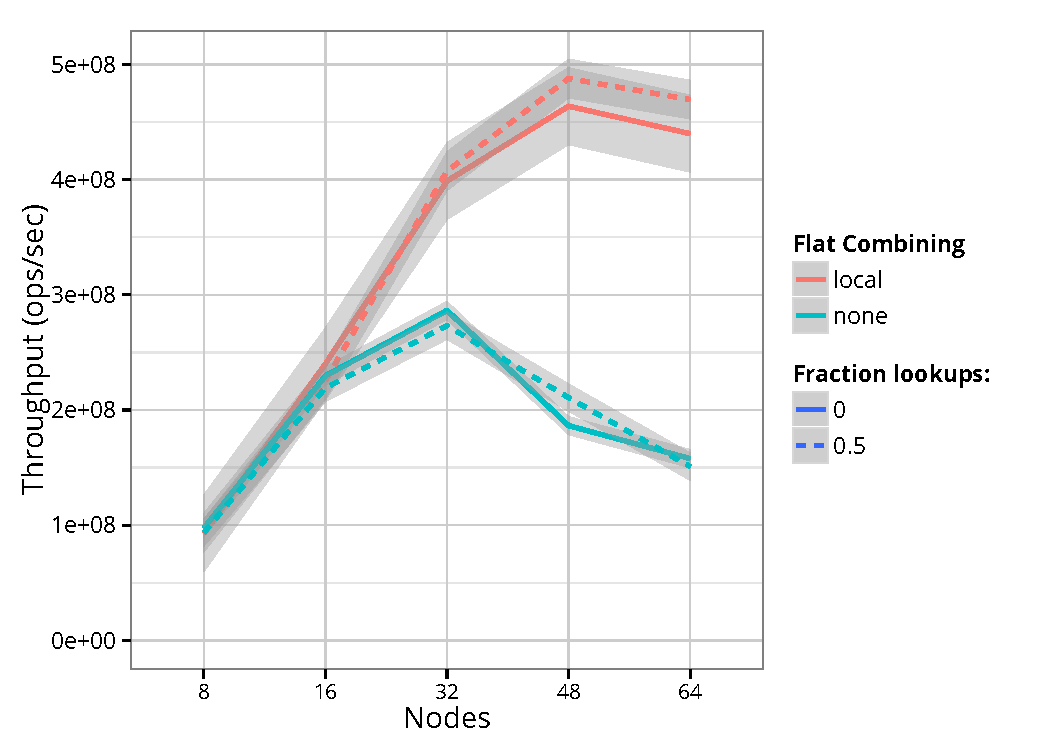
\includegraphics[width=\textwidth]{data/plots/hashmap_perf.pdf}
  % \caption{\emph{GlobalHashMap.} Same workload as for the Set, but random integers as the values in the map. Performance matches that of the Set.} \TODO{try increasing size of value "payload", currently is just a tiny int64.}
  % \label{fig:hashmap}
  % \end{subfigure}%
  %
%   \caption{
%     \emph{Raw performance of global data structures on simple throughput workloads.}
%     Results shown for workloads with varying mixtures of writing and reading operations. All experiments were performed with 16 cores per node, and a suitable set of Grappa runtime parameters fixed for a given plot.
%     \TODO{either all with error bars or none?}
%     \TODO{combine stack/queue \& set/map plots, no point in saying the same things twice.}
%   }\label{fig:datastructs}
% \end{figure*}

\paragraph{Queue and Stack}
The GlobalQueue and GlobalStack have very similar implementations in terms of how they are synchronized. Even with Grappa's aggregation, without combining, both the stack and queue completely fail to scale because of serialization of all workers' updates on the master core.
With combining, both scale well out to 64 nodes.
On the mixed workload, the stack is able to do matching locally, allowing it to reduce the amount of communication drastically, greatly improving its performance.

The queue also benefits from reduced synchronization and batching operations, and its all-push workload performs identically to the stack's.
However, the queue is unable to do matching locally, and in fact, the mixed workload performs worse because the current implementation serializes combined enqueue and dequeue operations. This restriction could be lifted with more careful synchronization at the master core allowing enqueues and dequeues to proceed in parallel as long as they do not conflict.

\paragraph{HashSet and HashMap}
The GlobalHashSet and GlobalHashMap have the same synchronization strategy (serialization happens at each hashed location) which allows them to scale fairly well even without combining because serialization only happens on conflicts. However, after 32 nodes, scaling drops off significantly due to increased number of concurrent accessors and more destinations.
The combining version is able to perform repeated inserts and repeated lookups with a single remote operation, enabling it to continue scaling further.

\subsection{Application Kernel Performance}
The original goal was to have scalable global data structures in the Grappa library that could be used in applications. Naive implementations of the data structures are insufficient for scaling, so HPC applications often implement their own highly customized versions. However, this forces each application to carefully reason about the ways in which the structures will be accessed. Additionally, many optimizations rely on relaxing global consistency in a way that does not affect the program. 
The Grappa data structures are synchronized to provide the most general use and match the expectations of programmers and algorithms.

\paragraph{Breadth-First Search}
\begin{figure}[t]
  \centering
  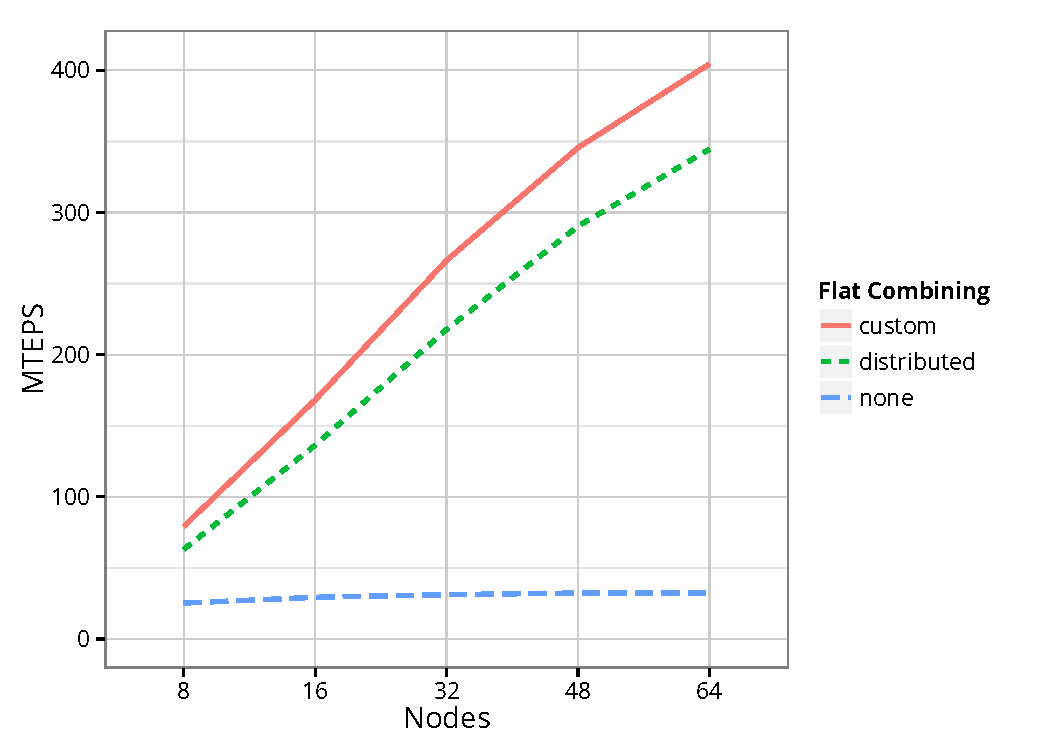
\includegraphics[width=0.5\textwidth]{data/plots/bfs_perf.pdf}
  \caption{\emph{BFS} on a Graph500-spec graph of scale 26 (64 million vertices, 1 billion edges), with the direction-optimizing BFS algorithm. Performance is measured in millions of Traversed Edges Per Second (MTEPS).}
  \label{fig:bfs_perf}
\end{figure}
The first application kernel is the Graph500 Breadth-First-Search (BFS) benchmark. This benchmark does a search starting from a random vertex in a synthetic graph and builds a search tree of parent vertices for each vertex traversed during the search. While this is a relatively simple problem, it exercises the random-access throughput of a system as well as being a primitive in many other graph algorithms. The BFS algorithm contains a global queue which represents the frontier of vertices to be visited in each level.
Our implementation employs the direction-optimizing algorithm by Beamer et al.\cite{Beamer:Graph500} which performs particularly well for the scale-free RMAT graphs generated by the benchmark.
The frontier queue in BFS is amenable to further optimization to take advantage of the fact that the algorithm does pushes and pops in separate phases, allowing consistency to be relaxed.
We compare our implementation of BFS using the flat-combined global queue described above with a highly tuned Grappa implementation that uses a custom asynchronous queue.

Figure~\ref{fig:bfs_perf} shows the results of scaling the BFS kernel up to 64 nodes. The simple queue implementation without flat combining is completely unscalable. However, the flat combining queue tracks the highly tuned asynchronous version. This illustrates that providing a safe, synchronized data structure for initially developing algorithms for PGAS is possible, while further optimizations can be applied incrementally.

\paragraph{Connected Components}
\begin{figure}[t]
  \centering
  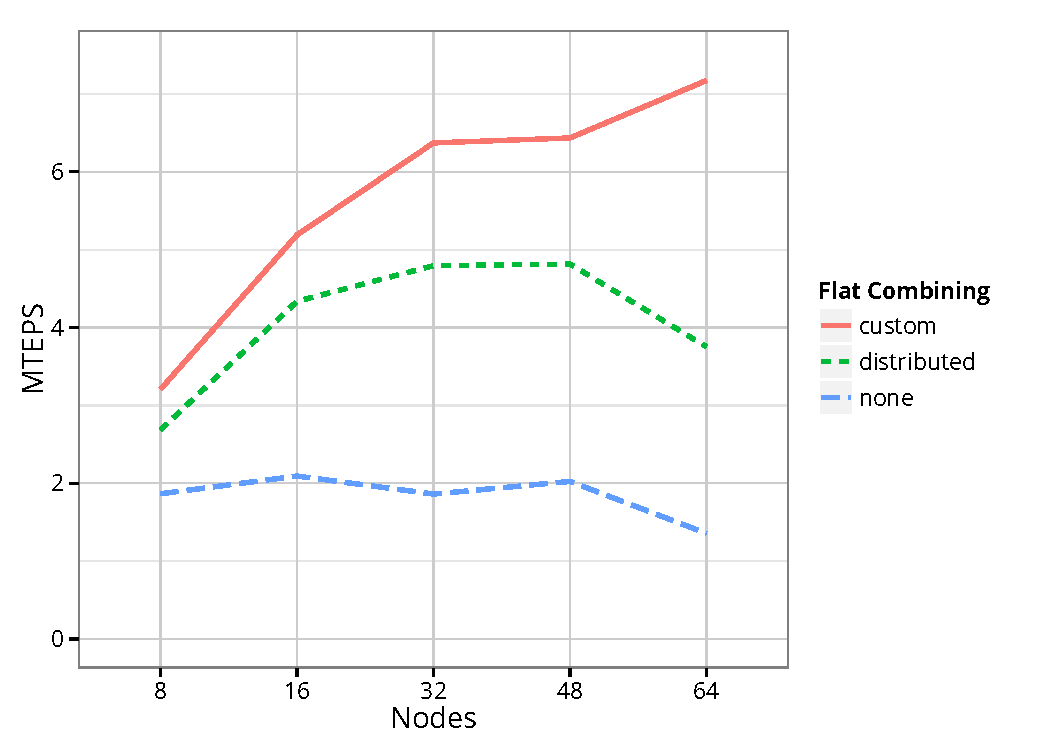
\includegraphics[width=0.5\textwidth]{data/plots/cc_perf.pdf}
  \caption{\emph{Connected Components} on the same scale 26 Graph500 graph. Performance is measured in MTEPS.}
  \label{fig:cc_perf}
\end{figure}
Connected Components (CC) is another simple graph analysis kernel that illustrates another use of global data structures in irregular applications. We implement the three-phase CC algorithm~\cite{mtgl} which was designed for the massively-parallel MTA-2 machine. In first phase, the algorithm begins many traversals in parallel from random starting vertices, labeling vertices with the root vertex. Whenever two traversals encounter each other, their searches are pruned and an edge between the two roots is inserted in a set. After all edges have been traversed in this way, the set of edges forms a new, typically much smaller, graph. The second phase performs the classical Shiloach-Vishkin parallel algorithm\cite{shiloach1982n} on this reduced graph, and the final phase propagates the component labels out to the full graph.
The creation of the reduced-graph edge set dominates the runtime of this algorithm, so improving the implementation of the set operations has a significant impact on performance. As in the case of BFS, further optimizations involving relaxation of consistency can be applied, in this case, to the global set. Therefore, we compare our straightforward implementation using the generic GlobalHashSet with and without flat combining against a tuned asynchronous implementation.

The results in Figure~\ref{fig::cc_perf} show that none of these three implementations scale very well out to 64 nodes. However, performing combining does improves the performance of the algorithm overall and improves scaling. The tuned version outperforms the synchronous version because it is able to build up most of the set locally on each core before merging them at the end of the first phase. An implementation of the GlobalHashSet that did not provide synchronized semantics could potentially relax consistency in a more general way, but this is left for future work.
